In questo capitolo sono presentate le principali tecnologie utilizzate durante lo sviluppo della tesi.
In primo luogo verrà presentata la piattaforma Hadoop con una veloce panoramica sulle sue principali feature.
Successivamente sarà trattato il framework Spark e le caratteristiche che lo hanno reso la 
soluzione con cui sono stati implementati gli algoritmi discussi in questa tesi.

\section{Hadoop}\label{sec:bd:hadoop}
Hadoop è un framework di natura open-source sviluppato da Apache.
Obiettivo della piattaforma è la gestione, elaborazione e memorizzazione di grandi quantità di dati in modo scalabile.

Hadoop si pone come alternativa rispetto al modello \textit{Massively Parallel Processor (MPP)}.
In questo paradigma vengono impiegati più processori, ciascuno avente le proprie risorse di memoria e disco.
Il lavoro complessivo è suddiviso in task.
Ciascun task è poi eseguito da un processore a seconda delle politiche di schedulazione del sistema.
Le architetture MPP sono composte da hardware e software proprietari.ù

Al contrario Hadoop è progettato per operare su commodity hardware e software open-source.
Il commodity hardware è l'insieme di tutte le componenti hardware già in possesso di un utente.
Tali componenti sono spesso generiche e senza particolari specifiche.
Ciò permette di poter integrare anche risorse di natura e caratteristiche differenti tra loro, senza per forza dover mantenere un omogeneità all'interno del sistema.
Questa diversità, oltre ad abbattere i costi, consente tempi di manutenzione e sostituzione più veloci.

Il framework Hadoop si compone di quattro moduli principali:

\begin{itemize}
    \item \textbf{HDFS}.
    \textit{File system} distribuito con alto throughput e replicazione a livello di blocco.
    \item \textbf{MapReduce} Framework per la creazione di applicazioni in grado di processare grandi moli di dati. 
    MapReduce è pensato per astrarre la complessità della gestione parallela della computazione.
    Per l'utente è necessario solamente specificare le fasi di Map (elaborazione parallela sui dati) e di reduce (aggregazione dei risultati).
    \item \textbf{Common}. Questo modulo contiene librerie e strumenti di utilità per la gestione del sistema.
    \item \textbf{YARN}. Framework per la gestione delle risorse all'intero del cluster Hadoop.
\end{itemize}

Oltre a questi sono disponibili ulteriori moduli accessori, illustrati in~\cref{fig:chap-6:hadoop-modules}.

\begin{figure}
    \centering
    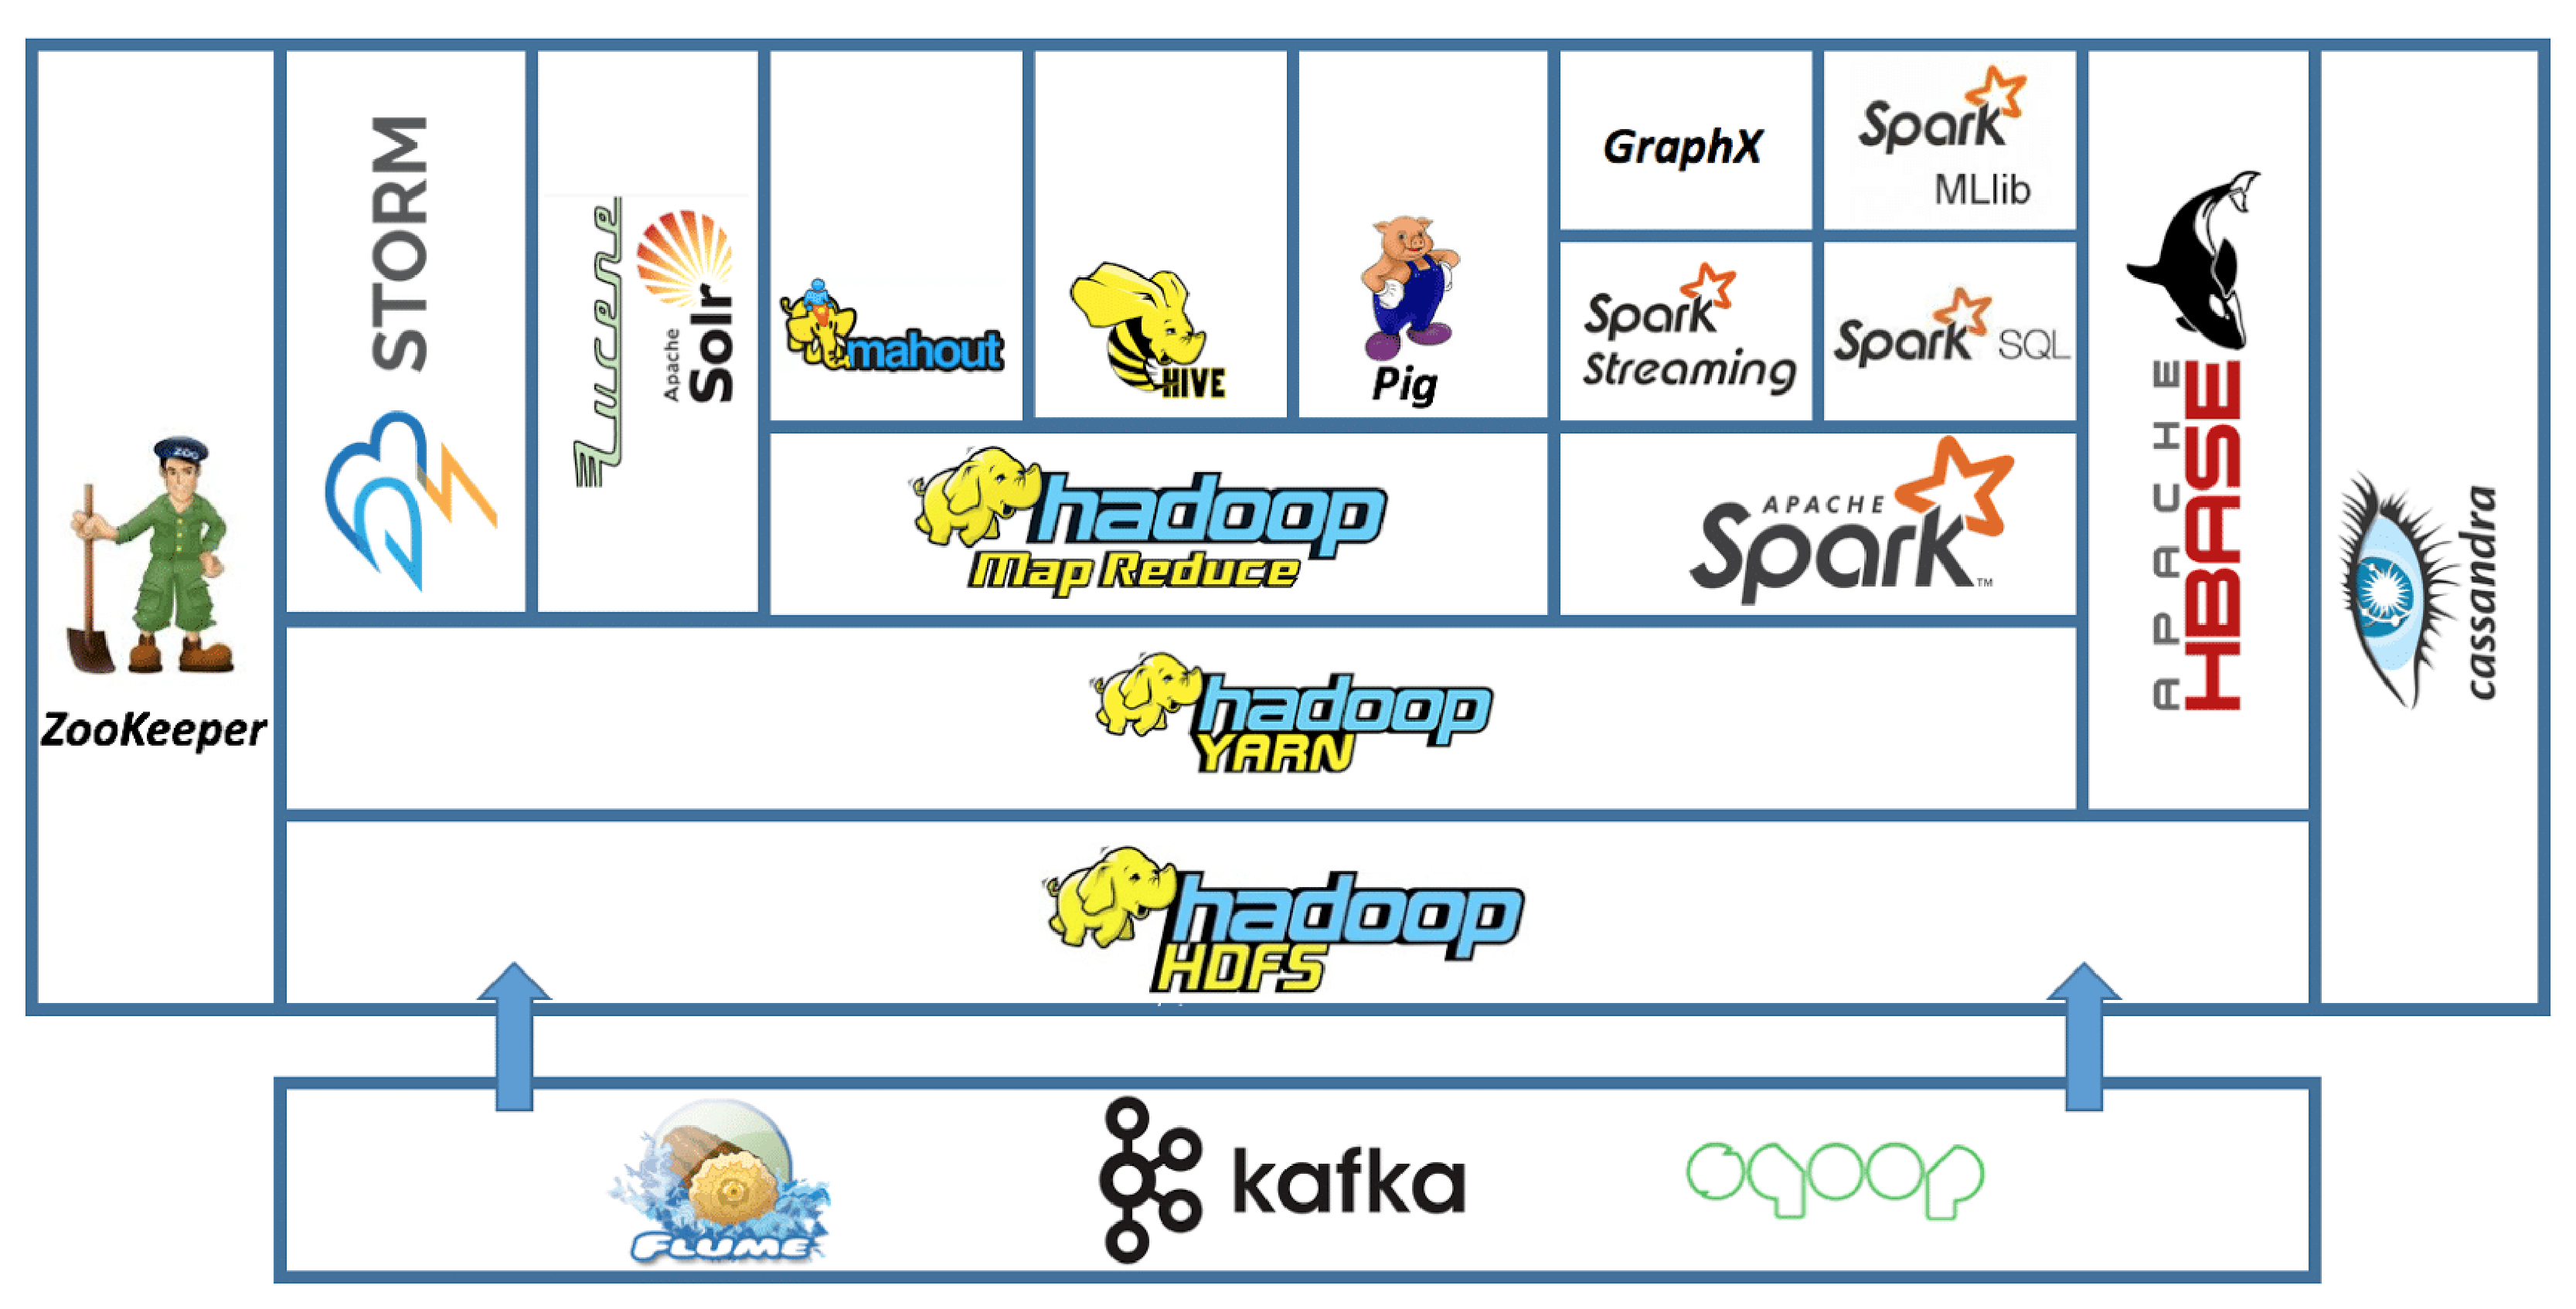
\includegraphics[width=\textwidth]{res/fig/sec-6/HadoopStack.pdf}
    \caption{Panoramica dell'ecosistema Hadoop, Fonte: \cite{Introduc53:online}}%
    \label{fig:chap-6:hadoop-modules}
\end{figure}

\subsection{HDFS}\label{subsec:db:hdfs}
HDFS, o Hadoop Distribuited File System, è il file system distribuito proprietario di Hadoop.
A differenza della maggior parte dei file system, Hadoop è progettato per operare con file di grandi dimensioni, introducendo politiche di ridondanza sui dati.
Il file system è stato progettato per operare in batch, ovvero raggruppando prima i dati, piuttosto che in streaming.
Questo tipo di accesso permette di ottenere un alto throughput, a discapito di una bassa latenza.
Alla luce di ciò, le applicazioni adottano un modello di accesso ai dati \textit{write-once-read-many}.

I principali punti forza di Hadoop sono:

\begin{itemize}
    \item \textbf{Computazione distribuita}.
    Nel momento in cui si tratta di computazione su grandi moli di dati, i costi per spostare i dati attraverso un'infrastruttura di rete possono peggiorare le performance del sistema.
    Per risolvere questo problema, Hadoop mette a disposizione delle interfacce per spostare la computazione negli stessi nodi, o quantomeno vicino, dove risiedono i dati da elaborare.
    Questo principio è noto col nome di data locality.
    
    \item \textbf{Resilienza ai guasti}.
    I guasti a livello hardware vanno considerati come naturali nella vita del sistema.
    Sotto questa prospettiva, HDFS mette in campo tecniche di identificazione dei guasti e di ripristino veloce e automatico dei processi.
    Grazie anche a questo meccanismo, è possibile gestire hardware differenti tra di loro.
    
    \item  \textbf{File system ottimizzato per file di grandi dimensioni}.
    HDFS definisce word, o blocchi in cui viene suddivisa e indicizzata la memoria del sistema, di dimensioni comprese tra 64 megabyte e un gigabyte.
    Blocchi di queste dimensioni gestiscono file nell'ordine di gigabyte o terabyte limitando il numero di blocchi in cui vengono divisi.
    Ciò implica una maggior coesione tra i dati, informazioni vicine e quindi con un alto grado di correlazione sono con buona probabilità salvate all'interno dello stesso blocco.
    
\end{itemize}

Passando poi all'architettura di HDFS, i nodi all'interno del sistema operano secondo un pattern master-slave.
Il master, chiamato NameNode, mantiene in modo persistente l'albero rappresentante il file system, insieme ai metadati collegati a cartelle e file.
Un altro compito del NameNode è mantenere il riferimento alla posizione di tutte le partizioni, o blocchi, di un certo file all'interno degli slave.
Infine il master si occupa delle operazioni di input/output sui file, come ad esempio le richieste di apertura, chiusura e cambio di nome.

Gli slave invece sono chiamati DataNode hanno il compito di salvataggio fisico e recupero dei blocchi di ogni file nel cluster.
I DataNode comunicano periodicamente con il NameNode, inviando l'elenco dei file e blocchi salvati sul singolo nodo.
Il master al contrario invia ai DataNodes comandi per la creazione e cancellazione di blocchi, che gli slave provvedono ad eseguire.

I singoli nodi sono poi organizzati in rack, che a loro volta sono organizzati in datacenter.
Questa struttura è rappresentata come un albero, avente nelle foglie i singoli nodi e nella radice il cluster.
La distanza tra due nodi, fondamentale per il principio di data locality, viene calcolata quindi come la distanza che i due nodi hanno nell'albero.

La struttura del cluster viene sfruttata anche durante il processo di ridondanza dei dati.
La replicazione dei dati migliora le performance di accesso ai dati e aumenta la robustezza del sistema.
La ridondanza avviene a livello di blocco: il NameNode mantiene in memoria la lista dei DataNode contenenti un certo blocco.
Il fattore di replica di default è impostato a 3.
Queste repliche sono salvate in nodi differenti del sistema aventi posizioni diverse.
La prima viene salvata sul nodo del client che ha lanciato il comando, la seconda in un nodo appartenente a un rack diverso del primo nodo, il terzo infine in un nodo nello stesso rack del secondo.

Le repliche possono essere ribilanciate in caso di problemi con un certo nodo o con un cambiamento nel cluster, ad esempio l'aggiunta di nuovi nodi.
Hadoop utilizza la topologia del cluster in combinazione con la replica dei blocchi per applicare il principio della data locality.
In primo luogo Hadoop cerca di mantenere la località a livello di nodo, poi a livello di rack, datacenter e infine cluster.

HDFS non ha performance efficienti quando viene richiesta una bassa latenza o i singoli file sono di dimensioni piccole.
La ragione è che HDFS è progettato per computazioni in ambito Big Data, in cui queste situazioni sono rare.

\subsection{YARN}\label{subsec:db:yarn}
YARN (Yet Another Resource Negotiator) è il gestore di risorse introdotto con Hadoop 2.0.
Originalmente sviluppato per migliorare le performance di MapReduce, YARN risulta abbastanza generico per adattarsi anche ad altri paradigmi.
Compito di questo gestore di risorse è negoziare le componenti necessarie per eseguire una certa applicazione e gestire la computazione distribuita.
YARN rimane trasparente all'utente: viene usato solamente da framework e mai direttamente dal codice dell'utente.

L'idea alla base di YARN è la separazione tra la gestione dei job e quella delle risorse.
Questa divisione è ulteriormente accentuata dalla presenza di due demoni che si occupano di questi aspetti.
YARN si compone di due processi demone:

\begin{itemize}
    \item \textbf{Resource Manager (RM)}.
    Demone globale, ne esiste solo uno per cluster, gestisce le risorse tra le varie applicazioni.
    Si compone di \textit{Scheduler} e \textit{Application Manager}.
    Il primo si occupa di allocare le risorse per le varie applicazioni, mentre il secondo è responsabile di accettare i job e eventualmente farli ripartire in caso di errori.
    \item \textbf{Node Manager (NM)}.
    Uno per ogni nodo slave, si occupa di eseguire i container.
    Un container è un'entità usata per eseguire un processo con un insieme limitato di risorse.
    Il Node Manager monitora l'esecuzione dei processi, il loro utilizzo di risorse e riporta i dati sul Resource Manager.
\end{itemize}

Nel momento in cui viene inviata al sistema la richiesta dell'esecuzione di una nuova applicazione, il RM cerca tra i vari NM uno che possa lanciare l'\textit{Application Master Process}.
A questo punto l'Application Manager negozia il primo container per eseguire l'AMP, che poi provvederà a richiedere le risorse necessarie.
Questo processo risulta altamente scalabile: RM infatti delega ai singoli AMP la richiesta delle risorse e di nuovi container.
In caso di fallimento inoltre è l'Application Master a occuparsi del ripristino.

YARN risulta quindi un framework aperto, che supporta altri paradigmi oltre a Map-Reduce, inoltre si integra bene con i meccanismi nativi di HDFS.

\subsection{Hive}\label{subsec:db:hive}
Hive è un modulo compatibile con Hadoop pensato per la lettura, scrittura e in generale gestione di dataset distribuiti.
Hive è costruito sulla base di Hadoop.

Funzionalità cardine del framework è la possibilità di interrogare i dati in un linguaggio proprietario Hive-QL.
Questo linguaggio si basa su una sintassi simil-SQL che produce query che vengono trasformate in serie di job Map-Reduce o Spark.

Altra feature rilevante è il supporto a molteplici tipi di dati.
Tra questi sono presenti CSV, Apache Parquet e Avro.
Il framework poi permette di accedere direttamente ai file salvati in HDFS.

\section{Spark}\label{sec:bd:spark}
Apache Spark è un framework per il calcolo distribuito e general purpouse.
Spark nasce dalle trasformazioni che gli hardware e i software hanno subito nel corso del tempo e dalle nuove esigenze emerse.
Negli ultimi anni sono disponibili macchine con CPU aventi sempre più core.
Oltre a questo è stato registrato anche un aumento della memoria ram nelle macchine.
Questo incremento ha permesso alla ram di divenire la memoria principale durante le computazioni, sostituendo il disco anche nella gestione di grandi moli di dati.
Dal punto di vista del software invece, è avvenuta un evoluzione che ha dato maggior rilevanza ai paradigmi funzionali rispetto a quelli ad oggetti.
Allo stesso modo i sistemi NoSQL, orientati a velocità e disponibilità hanno messo in ombra i classici sistemi SQL, orientati alla consistenza del dato.
Anche nel mondo Big Data sono emerse nuove possibilità ed esigenze: la necessità di poter processare dati in streaming, favorire approcci veloci e l'integrazione
con nuovi ambiti della data science, come ad esempio il machine learning sono alcuni esempi.

Alla luce di questi cambiamenti, Map-Reduce è divenuto limitante.
Questo paradigma infatti non si presta a tutti i tipi di elaborazione, essendo pensato per un approccio batch e basato sul disco.
Spark si pone come integrazione di Map-Reduce a queste nuove esigenze.
È in grado infatti di eseguire sia processi batch che streaming o query interattive.
Le sue primitive, basate sull'accesso a dati memorizzati in RAM, consentono performance cento volte più veloci di Map-Reduce.
Spark inoltre mantiene l'assoluta compatibilità con Hadoop tramite YARN e supporta varie fonti di dati, come ad esempio Hive.

\subsection{Architettura}\label{subsec:db:architecture}
Spark si basa su due principali astrazioni: RDD e DAG.

RDD, o \textit{Resilient Distribuited Dataset}, è la rappresentazione del framework Spark di una collezione di dati di qualunque natura.
Questa collezione è divisa in partizioni, ciascuna salvata su un nodo.
Un RDD può essere generato da qualunque fonte, ad esempio la query su un database esterno o la lettura di un file di input.

Le caratteristiche di un RDD sono le seguenti:

\begin{itemize}
    \item \textbf{Type inference}.
    Determina i tipi di dato durante la compilazione, senza bisogno di specificarli in fase di scrittura del codice.
    Questo è reso possibile dal linguaggio funzionale Scala, in cui è scritto il framework.
    
    \item \textbf{Cachability}.
    Gli RDD non sono di default salvati in memoria, ma sono processati e poi scartati.
    Per migliorare le performance, è possibile eseguire caching salvando in memoria o su disco un RDD.
    Ciò consente di evitare di doverlo ricalcolare ad ogni utilizzo.
    
    \item \textbf{Immutabilità}.
    Un RDD è per definizione immutabile.
    Qualunque operazione di trasformazione produce un nuovo RDD.
    Ciò semplifica la gestione di corse critiche senza bisogno di aggiungere nessun meccanismo di accesso alle risorse.
    
    \item \textbf{Laziness}.
    Le operazioni su un RDD possono essere di due tipi: trasformazioni o azioni.
    Le trasformazioni modificano i dati all'interno di un RDD, costruendone di fatto uno nuovo.
    Le azioni calcolano un risultato da restituire al driver o salvare su piattaforme esterne (ad esempio database Hive).
    Ogni operazione effettuata su un RDD non è eseguita fino alla richiesta di un azione.
    Le trasformazioni infatti producono metadati che vengono utilizzati nel momento in cui tramite un azione viene scatenata la catena di trasformazioni.

\end{itemize}

La proprietà di laziness pone le basi per la definizione di DAG.
Durante la computazione, a un RDD saranno associate più trasformazioni: queste possono essere rappresentate come un grafo.
Questo è chiamato lineage graph e costituisce la base per la definizione del piano di esecuzione.
Sulla base delle operazioni da eseguire e delle partizioni coinvolte, viene definito un piano di ottimizzazione.
Questo aggregherà operazioni diverse e sfrutterà il principio della data locality.

Una volta terminata la fase di ottimizzazione, il piano di esecuzione viene presentato nella forma di DAG (Directed Acyclic Graph).
DAG è un grafo i cui nodi sono RDD e gli archi le trasformazioni che portano da un RDD all'altro.
Il grafo è direzionato e sono assenti cicli al suo interno.

Determinato il DAG, questo viene diviso in stage secondo il seguente principio: si raggruppano operazioni fino a giungere a una trasformazione che richieda un processo di shuffle dei dati.
Uno shuffle è un operazione di collezione e ridistribuzione dei dati necessaria per certe istruzioni, come ad esempio un raggruppamento dei dati su una certa chiave.
A questo punto lo stage termina e ne viene creato uno nuovo.
Ogni stage è poi diviso in task in numero pari a quello delle partizioni moltiplicato per il numero delle trasformazioni da eseguire.
Ogni task è assegnato a un nodo con il principio della data locality, avendo però attenzione di non sovraccaricare il sistema.
In caso di problemi, un task può essere schedulato su nodi differenti in modo da prevenire blocchi e ritardi.

Trattando infine dell'architettura di Spark, il paradigma adottato è ancora una volta master-slave.
Di seguito sono trattati i principali componenti dell'architettura di Spark:

\begin{itemize}
    \item \textbf{Driver}.
    Master dell'architettura, unico nell'applicazione. 
    Gestisce le fasi della creazione e ottimizzazione di DAG, inoltre assegna i task ai vari executor.
    
    \item \textbf{Executor}.
    Processo avente il compito di eseguire su ogni core un task.
    Ad ogni applicazione possono essere assegnati più executor, ciascuno avente una certa quantità di RAM e un numero fissato di CPU.
    
    \item \textbf{Cluster Manager}.
    Componente che si occupa delle risorse.
    Può essere un processo stanalone o un resource manager compatibile con Spark, come ad esempio YARN.
\end{itemize}

\subsection{SparkSQL}\label{subsec:db:sparksql}
Spark SQL è un modulo costruito sopra Spark.
Obbiettivo di Spark SQL è quello di poter integrare l'elaborazione di dati strutturati e semi-strutturati tramite primitive simili al linguaggio SQL.
La necessità alla base di Spark SQL è stata l'integrazione di computazione procedurale e query SQL su database di grandi dimensioni.
Spark SQL nasce quindi come modulo che integra le API procedurali con il modello relazionale.
Altri punti fondamentali per Spark SQL sono l'efficienza nelle operazioni e il supporto a diversi database esterni.

Posti questi obbiettivi, il framework Spark SQL fornisce:

\begin{itemize}
    \item \textbf{Integrazione}.
    Spark SQL permette di interrogare strutture dati all'interno delle applicazioni Spark.
    Queste interrogazioni possono essere fatte o tramite API su RDD o con query SQL.
    Il framework è disponibile per i linguaggi in cui è disponibile Spark.
    \item \textbf{Compatibilità con Hive}.
    Viene supportata la sintassi di HiveQL ed è totale la compatibilità con i dati, le query e le user defined function su Hive. 
    \item \textbf{Connettività Standard}.
    Vengono supportati gli standard industriali JDBC e ODBC.
    \item \textbf{Accesso Uniforme ai dati}.
    Sono supportate diverse fonti di dati, come ad esempio Hive, Avro, JSON o Parquet.
    Questi dati sono trattati nella stessa maniera e, una volta caricati, possono essere integrati tra di loro.
    \item \textbf{Scalabilità}.
    Spark SQL combina la laziness del modello RDD di Spark con una gestione colonnare e un ottimizzatore interno di query per migliorare i risultati.
\end{itemize}

La caratteristica principale di Spark SQL è la definizione di una nuova astrazione, chiamata Dataframe.
Un Dataframe è una collezione di dati distribuita organizzata in colonne, rendendolo di fatto equivalente a una tabella relazionale.
Questa astrazione è basata su RDD, ne conserva quindi tutte le proprietà e modalità di computazione.

